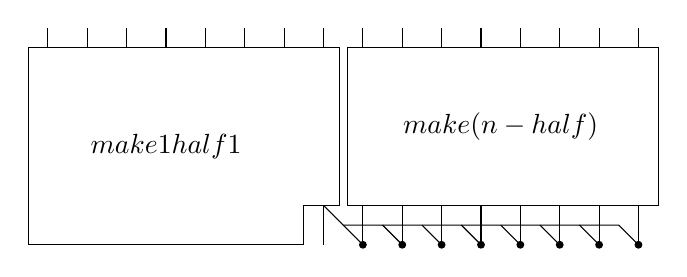
\begin{tikzpicture}
\begin{scope}[scale=.5]
  \draw (0.5, 0) -- (7.5, 0) -- (7.5, 1) -- (8.4, 1) -- (8.4, 5) -- (0.5, 5) -- cycle ;
  \draw (8.6, 1) -- (16.5, 1) -- (16.5, 5) -- (8.6, 5) -- cycle ;
  \foreach \x in {1, ...,16}
    \draw (\x, 5) -- (\x, 5.5) ;
  \foreach \x in {8, ...,16}
    \draw (\x, 0) -- (\x, 1) ;
  \draw (8, 1) -- (8.5, .5) -- (15.5, .5);
  \foreach \x in {9, ...,16} {
    \draw (\x-.5, .5) -- (\x, 0);
    \fill (\x, 0) circle (.1);
  }
  \node at (4, 2.5) {\lst$make1 half 1$};
  \node at (12.5, 3) {\lst$make (n - half)$};
\end{scope}
\end{tikzpicture}
